\nxsection{Le R\^ole ''Magasinier''}\label{sec:utilisateurs-lemagasinier}
\index{magasinier}
\index{LeMagasinier}

La figure~\ref{fig:yeren-fenetre-magasinier} illustre
la fen\^etre d'acceuil d'un utilisateur avec le
\role \magasinier, apr\`es qu'il se soit enregistr\'e
dans \yeroth.\\

\begin{figure}[!htbp]
\centering
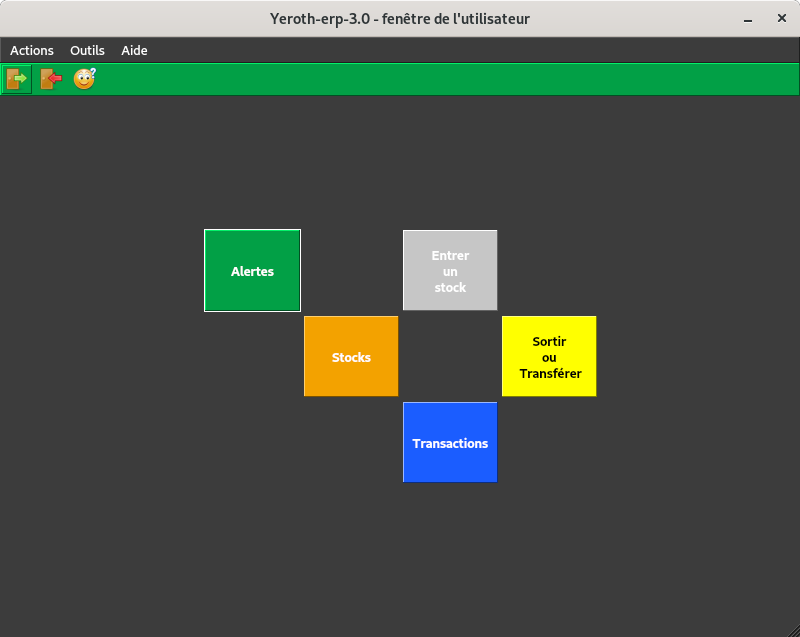
\includegraphics[scale=0.63]{images/yeren-fenetre-magasinier.png}
\caption{La fen\^etre d'acceuil d'un \magasinier.}
\label{fig:yeren-fenetre-magasinier}
\end{figure}

Un utilisateur de \yeroth avec le \role \magasinier a acc\`es
aux fonctionnalit\'es suivantes:

\begin{enumerate}[1)]
	\item gestion des stocks (voir chapitre~\ref{chap:gestion-stocks})
	\item mouvements de stocks (voir chapitre~\ref{chap:mouvements-de-stocks})	
	\item syst\`eme d'alertes (voir chapitre~\ref{chap:systeme-dalertes}).\\
\end{enumerate}
